\chapter{HASIL DAN PEMBAHASAN}
\vspace{1em}

\section{Hasil dan Pembahasan Sistem}
\subsection{Hasil dan Pembahasan Implementasi pada Robot}
Pada tahap ini dilakukan implementasi sistem ke dalam robot humanoid ROBOTIS-OP3 untuk mereplikasi gerakan manusia berdasarkan hasil estimasi pose yang telah diolah sebelumnya. Proses ini melibatkan beberapa tahapan penting, mulai dari konversi data pose 3D menjadi sudut servo, validasi area pergerakan robot, hingga eksekusi gerakan secara fisik. Berikut adalah pembahasan hasil implementasi pada masing-masing tahap.
\subsubsection{Konversi Koordinat ke Sudut Servo}

\begin{figure}[H]
    \centering
    \includegraphics[width=0.7\textwidth]{images/angles_per_joint.png}
    \caption{Grafik perubahan sudut sendi robot per frame pada lengan kiri, lengan kanan, dan kepala}
    \label{fig:angles_per_joint}
\end{figure}

Gambar~\ref{fig:angles_per_joint} menunjukkan hasil visualisasi perubahan sudut sendi (servo) pada robot humanoid untuk mengontrol pergerakan lengan kiri, lengan kanan, dan kepala dalam satu sekuens gerakan tari tradisional. Tari tersebut melakukan gerakan menekuk lengan secara bergantian dengan kepala menengok ke kanan dan ke kiri secara bergantian.

Grafik bagian atas memperlihatkan \emph{Left Arm Angles}, yaitu perubahan sudut pada \emph{Shoulder Pitch}, \emph{Shoulder Roll}, \emph{Elbow Pitch}, dan \emph{Elbow Roll} di lengan kiri. Kurva menunjukkan variasi sudut yang mencerminkan pergerakan lengan naik, turun, dan rotasi sepanjang gerakan.

Grafik bagian tengah menampilkan \emph{Right Arm Angles}, dengan pola perubahan sudut serupa pada lengan kanan. Terlihat perubahan signifikan pada sudut \emph{Elbow Pitch} dan \emph{Elbow Roll}, terutama pada rentang frame 50 hingga 150 yang menandai fase gerakan tangan intens.

Grafik bagian bawah memperlihatkan \emph{Head Angles}, yaitu perubahan sudut kepala pada tiga sumbu: \emph{Head Pan} (rotasi mendatar), \emph{Head Pitch} (mendongak atau menunduk), dan \emph{Head Roll} (kemiringan samping). Meskipun variasinya lebih kecil dibandingkan pergerakan lengan, grafik ini tetap menunjukkan dinamika gerakan kepala sesuai dengan input pose.

Secara keseluruhan, visualisasi ini menunjukkan bahwa sistem berhasil mengonversi data pose 3D menjadi perintah sudut servo yang halus, kontinu, dan sesuai dengan variasi gerakan tari. Pola sudut yang stabil dan tidak fluktuatif secara ekstrem mendukung proses eksekusi gerakan robot secara natural dan aman.


\subsection{\textit{Motion Imitation} Pada Robot}

Pada hasil \textit{motion imitation}, dilakukan dua jenis percobaan untuk menguji sistem. Percobaan pertama dilakukan dengan input gambar berpose khusus untuk menguji cakupan pergerakan robot. Input ini meliputi berbagai variasi gerakan seperti tangan merentang ke samping (\textit{T-pose}), tangan ke depan, tangan ke atas, dan kombinasi lainnya yang mencakup area maksimal pergerakan lengan dan kepala robot. Percobaan ini bertujuan untuk mengetahui seberapa baik sistem dapat memetakan berbagai pose manusia ke dalam ruang gerak (range of motion) robot ROBOTIS-OP3.

Percobaan kedua dilakukan pada gerakan tari tradisional, dengan rangkaian gerakan yang lebih dinamis dan variatif. Hasil percobaan ditunjukkan dengan menampilkan tiga komponen utama secara berdampingan dalam satu gambar, yaitu frame asli, hasil estimasi rangka 3D, dan gerakan robot yang menirukan pose. Gambar berikut memperlihatkan contoh rangkaian gerakan tari tradisional yang diproses oleh sistem.

Pada gambar bagian kiri ditampilkan frame video input yang menjadi dasar proses estimasi pose. Bagian tengah menunjukkan hasil prediksi koordinat 3D yang divisualisasikan dalam bentuk rangka, sedangkan bagian kanan memperlihatkan robot humanoid ROBOTIS-OP3 yang menjalankan pose hasil konversi sudut sendi.

\begin{figure}[H]
    \centering
    \includegraphics[width=\textwidth]{images/hasil.jpg}
    \caption{Visualisasi motion imitation pada gerakan tari tradisional: frame video asli, rangka hasil estimasi 3D, dan gerakan robot}
    \label{fig:motion_imitation_tari}
\end{figure}

Pada Gambar~\ref{fig:motion_imitation_tari}, ditampilkan hasil percobaan \textit{motion imitation} pada gerakan tari tradisional, yaitu tari Denok Semarangan. Robot berhasil menirukan gerakan tari dengan cukup baik, terutama pada pergerakan tangan dan kepala yang menjadi fokus utama dalam penelitian ini. Posisi lengan dan kepala robot mengikuti pola pose dari data rangka secara real-time, dengan pergerakan yang halus dan stabil antar frame.

\begin{figure}[H]
    \centering
    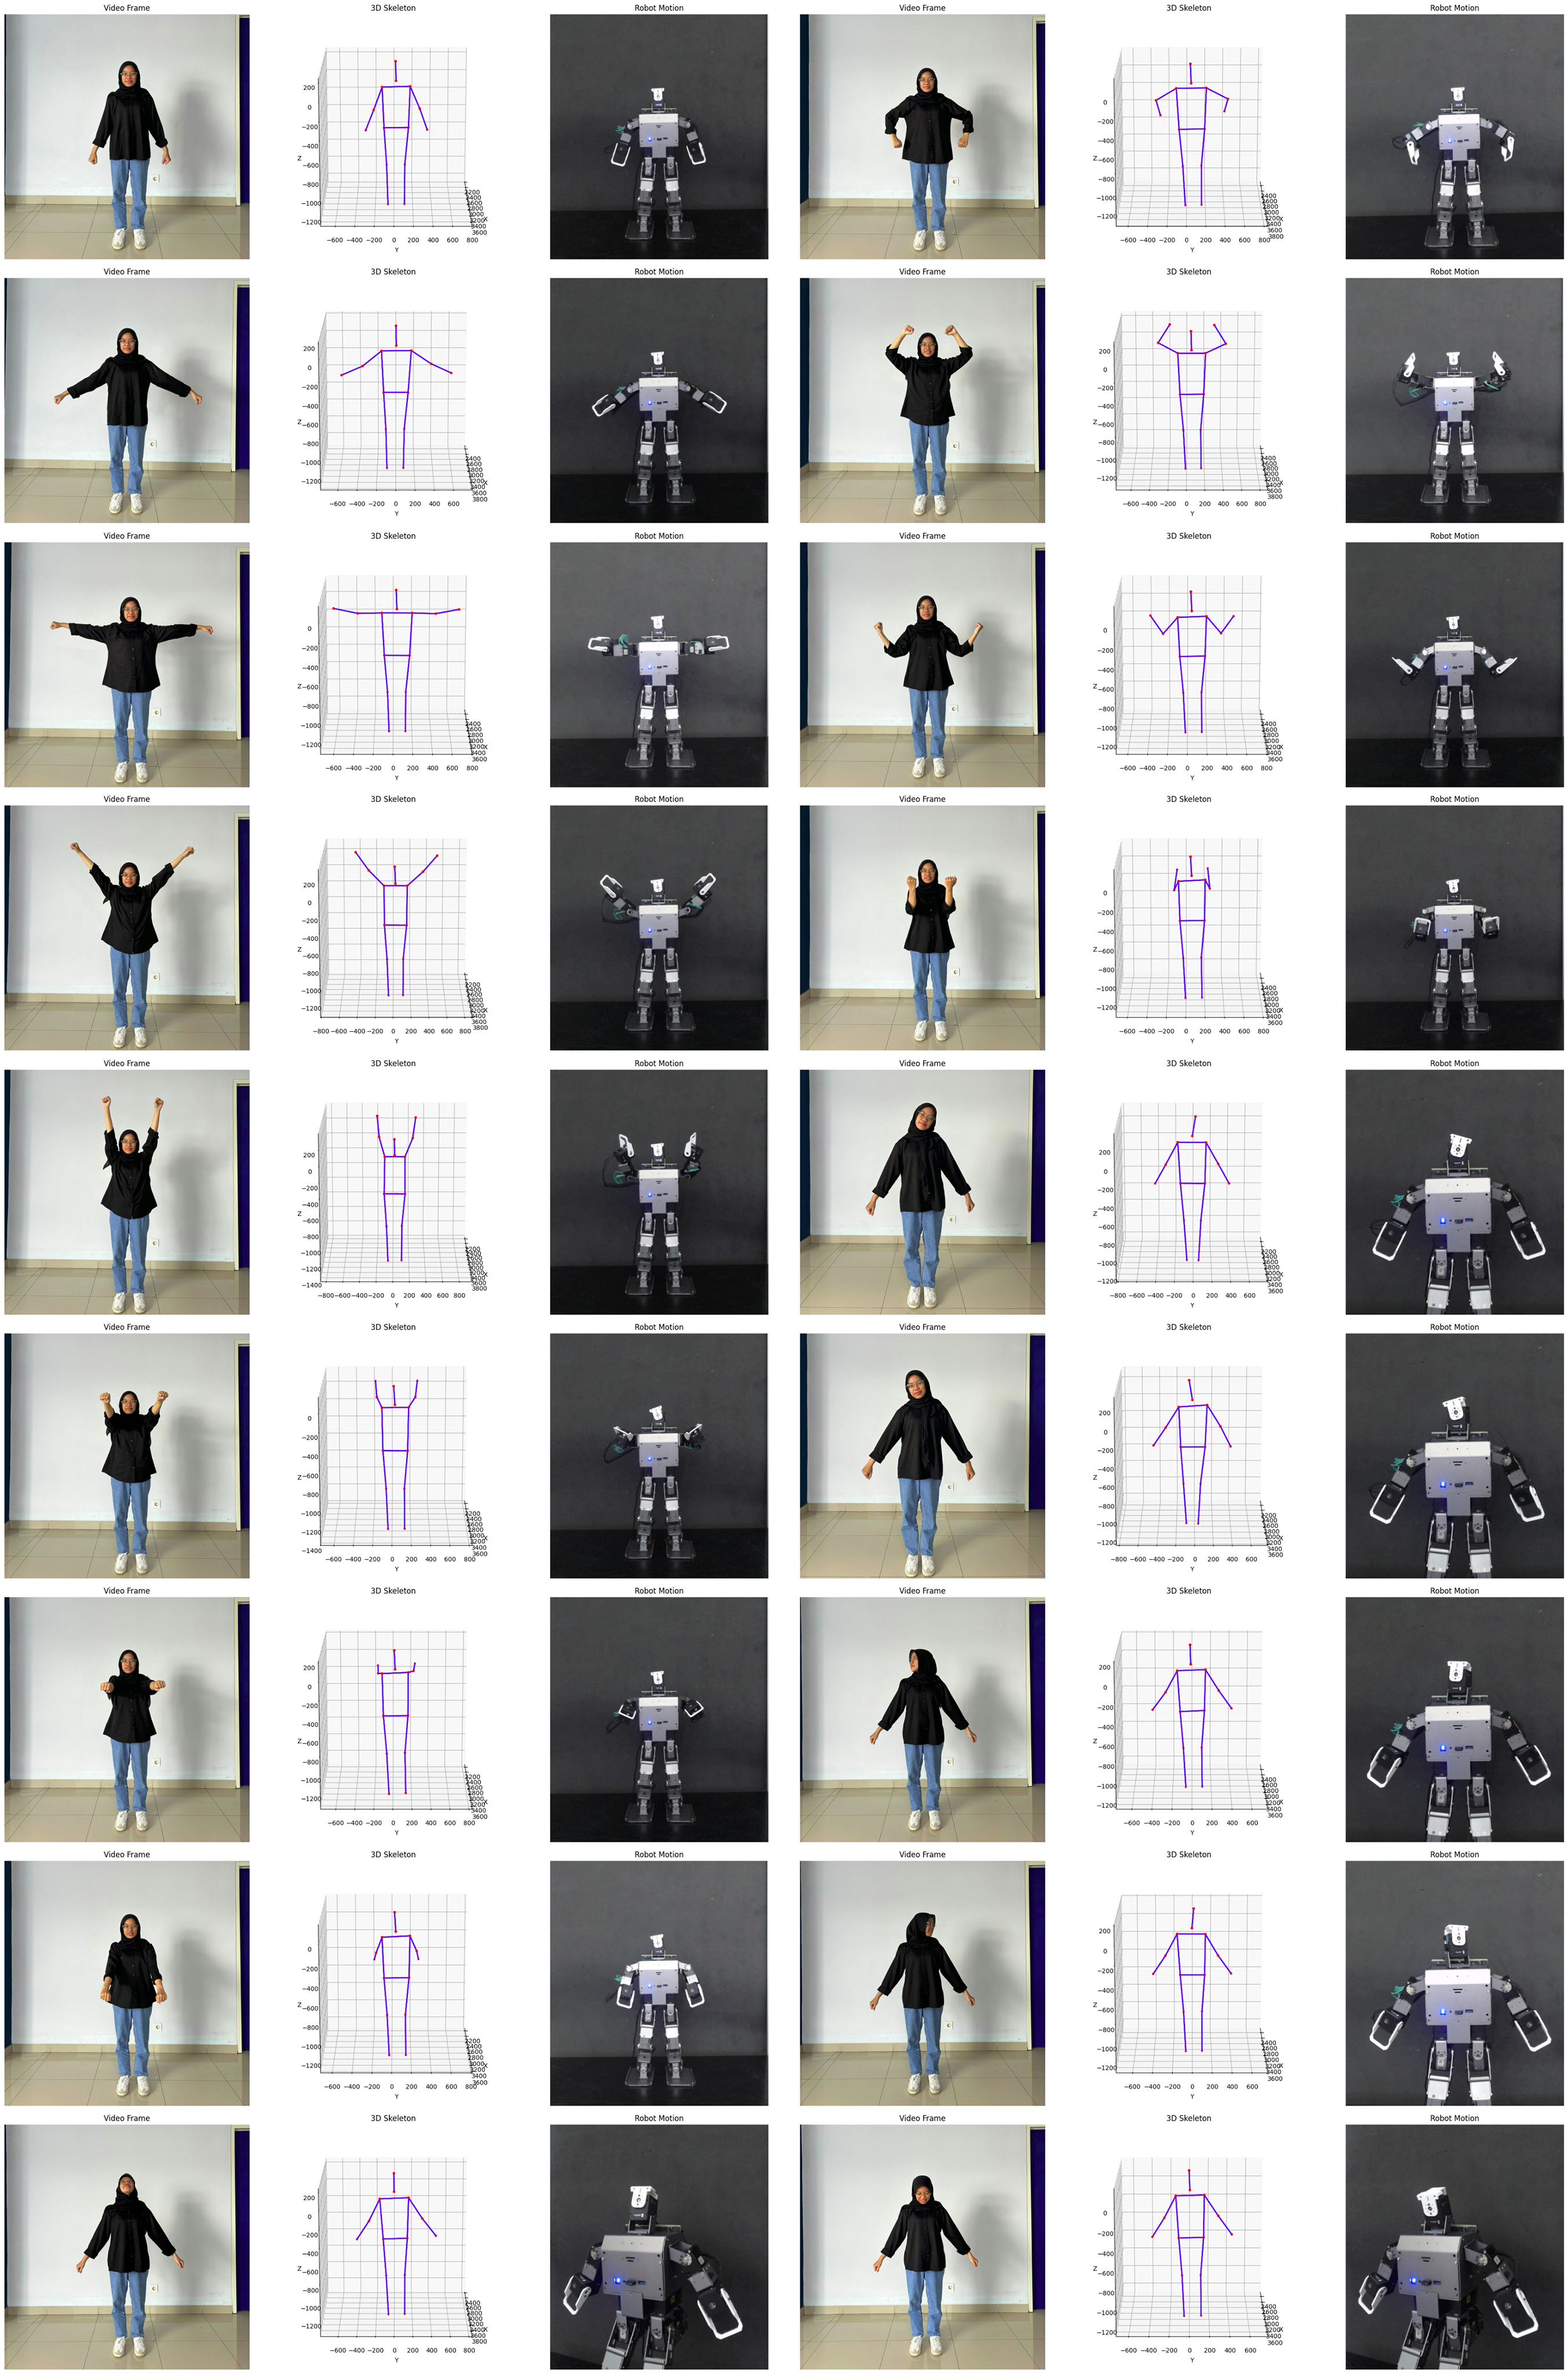
\includegraphics[width=\textwidth]{images/motion_imitation_coverage.png}
    \caption{Visualisasi motion imitation untuk cakupan gerakan: frame video asli, rangka hasil estimasi 3D, dan gerakan robot}
    \label{fig:motion_imitation_coverage}
\end{figure}

Berdasarkan Gambar~\ref{fig:motion_imitation_coverage}, dapat dilihat bahwa robot mampu mengikuti berbagai variasi gerakan dengan baik. Pada pengujian cakupan gerakan, sistem berhasil memetakan gerakan lengan seperti merentang ke samping, mengangkat ke atas, dan mengarah ke depan tanpa melebihi batas pergerakan mekanis robot. Gerakan yang dihasilkan tetap stabil dan tidak terdapat pergerakan yang melebihi limit servo, sehingga sistem berhasil menjaga keamanan aktuator. Hal ini menunjukkan bahwa proses \textit{motion retargeting} telah berhasil menyesuaikan koordinat tubuh manusia dengan batas kemampuan robot ROBOTIS-OP3 secara efektif.

Walaupun terdapat perbedaan proporsi anatomi antara manusia dan robot, sistem tetap mampu menghasilkan gerakan yang menyerupai tari tradisional secara visual. Hasil ini menunjukkan bahwa pipeline mulai dari input video, estimasi rangka 3D, konversi sudut sendi, hingga eksekusi gerakan robot berjalan dengan baik secara \textit{end-to-end}.


\subsection{Hasil dan Pembahasan Fungsional Sistem}

Pengujian fungsional sistem dilakukan untuk memastikan bahwa seluruh fitur utama berjalan sesuai spesifikasi yang telah dirancang. Pengujian telah dilakukan oleh anggota tim robotik terhadap aplikasi yang telah dikembangkan. Terdapat 6 fitur utama dengan total 6 skenario pengujian, dan seluruh skenario berhasil dijalankan tanpa kendala. Persentase keberhasilan pengujian fungsional sistem adalah \(\frac{6}{6} \times 100\% = 100\%\). Dengan demikian, seluruh fitur pada sistem dinyatakan telah memenuhi kebutuhan fungsional sesuai perancangan.

Tabel~\ref{tab:hasil_pengujian_fungsional} berikut menyajikan hasil lengkap pengujian fungsional sistem.


\begin{longtable}{|c|p{2.5cm}|p{3cm}|p{3cm}|p{2.5cm}|}
\caption{Hasil Pengujian Fungsional Sistem} \label{tab:hasil_pengujian_fungsional} \\
\hline
\textbf{No} & \textbf{Fitur} & \textbf{Skenario Pengujian} & \textbf{Hasil Pengujian} & \textbf{Kesimpulan} \\ \hline
\endfirsthead
\hline
\textbf{No} & \textbf{Fitur} & \textbf{Skenario Pengujian} & \textbf{Hasil Pengujian} & \textbf{Kesimpulan} \\ \hline
\endhead

1 & Upload Video & Pengguna mengunggah file video gerakan tari tradisional & File video berhasil diunggah & Berhasil \\ \hline
2 & Estimasi Pose dan Filtering & Pengguna menekan tombol \textit{Start Pose Estimation} & \textit{Pose estimation} berhasil dijalankan & Berhasil \\ \hline
3 & Tampilan Estimasi Pose & Sistem menampilkan skeleton 3D pada setiap frame video & Sistem menampilkan skeleton 3D dari video (frame awal hingga frame akhir) & Berhasil \\ \hline
4 & Status Log & Sistem mencatat proses pada area log setiap tahapannya & Sistem menampilkan setiap proses yang berlangsung & Berhasil \\ \hline
5 & Penyimpanan Data & Pengguna menyimpan hasil estimasi ke dalam file JSON & File estimasi dari setiap frame didapatkan dalam bentuk JSON & Berhasil \\ \hline
6 & Playback Robot & Pengguna menekan tombol \textit{Gerak} untuk menjalankan robot & Robot bergerak sesuai hasil estimasi proses sebelumnya & Berhasil \\ \hline

\end{longtable}
Dari hasil pengujian fungsional, dapat disimpulkan bahwa sistem telah memenuhi seluruh kebutuhan fungsi utama yang dirancang. Proses mulai dari input video, estimasi pose, penyimpanan data, hingga eksekusi gerakan pada robot ROBOTIS-OP3 berhasil dijalankan dengan baik tanpa kendala teknis.

Keberhasilan ini menunjukkan bahwa sistem dapat digunakan sebagai media representasi gerakan tari tradisional secara otomatis melalui robot humanoid. Implementasi \textit{black-box testing} berhasil memvalidasi bahwa alur aplikasi sesuai dengan rancangan antarmuka dan kebutuhan operasional.

\subsection{Hasil dan Pembahasan Performa Model}

Bagian ini menjelaskan hasil pengujian performa model DeciWatch, mencakup proses training, perbandingan performa antar model, serta visualisasi hasil estimasi pose dan pergerakan sudut sendi.

\subsubsection{Proses Pelatihan dan Evaluasi Model}

Model DeciWatch dilatih menggunakan dataset AIST++ dalam dua sesi training dengan total 45 epoch. Tujuan pelatihan adalah untuk meningkatkan akurasi estimasi pose 3D secara temporal dengan mengoreksi prediksi awal dari model baseline. Pelatihan dilakukan dengan GPU NVIDIA RTX 3060 Mobile. Sesi pertama berlangsung selama 20 epoch, sedangkan sesi kedua dilakukan dari epoch ke-21 hingga ke-45 dengan memuat parameter dari sesi sebelumnya.

Selama proses training, dicatat nilai loss dan Mean Per Joint Position Error (MPJPE). MPJPE input berasal dari prediksi awal model SPIN (yang tetap konstan karena tidak dilatih ulang), sedangkan MPJPE output dihasilkan dari model DeciWatch setelah proses filtering temporal.
\begin{enumerate}
    \item {Sesi Pertama (Epoch 1--20)} \\
    Pada sesi pertama, model dilatih selama 20 epoch. Gambar~\ref{fig:loss_lr_epoch_1} menunjukkan penurunan loss secara konsisten seiring dengan penurunan \textit{learning rate} menggunakan skema eksponensial decay sebesar 0{,}95 per epoch.

    \begin{figure}[H]
        \centering
        \includegraphics[width=0.9\textwidth]{images/loss_lr_vs_epoch.png}
        \caption{Perbandingan nilai loss dan learning rate terhadap epoch (1--20)}
        \label{fig:loss_lr_epoch_1}
    \end{figure}

    Gambar~\ref{fig:mpjpe_epoch_1} memperlihatkan tren penurunan MPJPE output secara bertahap, sementara MPJPE input tetap konstan. Hal ini menunjukkan bahwa DeciWatch mulai berhasil mengurangi error prediksi pada sesi pertama.

    \begin{figure}[H]
        \centering
        \includegraphics[width=0.9\textwidth]{images/mpjpe_vs_epoch.png}
        \caption{Perbandingan MPJPE antara input dan output pada sesi pelatihan pertama}
        \label{fig:mpjpe_epoch_1}
    \end{figure}

    \item {Sesi Kedua (Epoch 21--45)} \\
    Pada sesi kedua, proses pelatihan dilanjutkan dengan memuat parameter dari sesi pertama. Gambar~\ref{fig:loss_lr_epoch_2} menunjukkan bahwa penurunan loss tetap berlanjut, meskipun laju penurunannya lebih kecil karena \textit{learning rate} terus berkurang.

    \begin{figure}[H]
        \centering
        \includegraphics[width=0.9\textwidth]{images/loss_lr_vs_epoch_2.png}
        \caption{Perbandingan nilai loss dan learning rate terhadap epoch (21--45)}
        \label{fig:loss_lr_epoch_2}
    \end{figure}

    Gambar~\ref{fig:mpjpe_epoch_2} memperlihatkan penurunan MPJPE output yang konsisten hingga epoch ke-45. Ini menunjukkan bahwa model semakin mampu mengoreksi kesalahan prediksi secara temporal.

    \begin{figure}[H]
        \centering
        \includegraphics[width=0.9\textwidth]{images/mpjpe_vs_epoch_2.png}
        \caption{Perbandingan MPJPE antara input dan output pada sesi pelatihan kedua}
        \label{fig:mpjpe_epoch_2}
    \end{figure}
\end{enumerate}

Tabel~\ref{tab:hasil_training} merangkum hasil akhir dari dua sesi training, termasuk MPJPE output, loss akhir, dan durasi pelatihan. Berdasarkan tabel tersebut, dapat dilihat bahwa model berhasil menurunkan MPJPE output dari 66{,}10 mm menjadi 64{,}98 mm dengan penurunan loss dari 0{,}1666 ke 0{,}1522 selama dua sesi pelatihan.

\begin{table}[H]
\centering
\caption{Ringkasan Hasil Pengujian Training Model DeciWatch}
\label{tab:hasil_training}
\begin{tabular}{|c|c|c|c|c|}
\hline
\textbf{Sesi} & \textbf{Epoch} & \textbf{MPJPE Output (mm)} & \textbf{Loss Akhir} & \textbf{Durasi Training} \\ \hline
1 & 1--20  & 66.10 & 0.1666 & 24 jam \\ \hline
2 & 21--45 & 64.98 & 0.1522 & 26 jam \\ \hline
\end{tabular}
\end{table}




\subsubsection{Visualisasi Perbandingan Koordinat 3D}
Visualisasi hasil prediksi dilakukan untuk membandingkan koordinat 3D antara model baseline (Metrabs) dan DeciWatch. Grafik berikut menunjukkan perbandingan koordinat X, Y, dan Z untuk beberapa joint seperti pergelangan tangan kanan (\textit{rwrist}), pergelakngan tangan kiri (\textit{lwrist}), dan kepala (\textit{head}).

\begin{figure}[H]
    \centering
    \includegraphics[width=\textwidth]{images/koordinat_per_joint.png}
    \caption{Perbandingan koordinat X, Y, dan Z hasil estimasi pose 3D antara Metrabs (\textit{Raw}) dan DeciWatch (\textit{Filtered})}
    \label{fig:koordinat_joint}
\end{figure}

Kurva berwarna merah menunjukkan data mentah dari Metrabs, sedangkan kurva hijau menunjukkan hasil DeciWatch. Berdasarkan visualisasi tersebut, dapat dilihat bahwa pada data mentah (\textit{Raw}), khususnya pada sumbu Z, terdapat fluktuasi yang lebih signifikan dibandingkan sumbu X dan Y. Hal ini disebabkan karena sumbu Z merepresentasikan kedalaman (\textit{depth}), yang merupakan komponen paling sulit diprediksi dari input 2D. Model estimasi pose seperti Metrabs harus mengonversi informasi gambar dua dimensi menjadi prediksi posisi tiga dimensi, sehingga prediksi pada sumbu Z cenderung lebih rentan terhadap noise.

Dengan penerapan DeciWatch sebagai model \textit{temporal filter}, noise pada sumbu Z berhasil direduksi secara signifikan. DeciWatch memanfaatkan konteks waktu untuk melakukan \textit{smoothing} pada urutan pose, sehingga menghasilkan data gerakan yang lebih halus dan stabil. Hal ini penting agar proses konversi ke sudut sendi (melalui \textit{inverse kinematics}) menjadi lebih akurat dan menghindari gerakan robot yang tidak realistis akibat data yang terlalu berfluktuasi.


\subsubsection{Perbandingan Model Custom dan Pre-trained}

Pengujian dilakukan untuk membandingkan performa model DeciWatch hasil training custom dengan model pre-trained bawaan DeciWatch. Model custom menggunakan \textit{skip frame} 5, sedangkan model pre-trained menggunakan nilai default 10.

Hasil perbandingan menunjukkan bahwa model custom memiliki MPJPE output lebih rendah, yaitu 64{,}98 mm dibandingkan pre-trained sebesar 71{,}27 mm. Hal ini disebabkan oleh resolusi temporal yang lebih rapat pada model custom, sehingga mampu mempelajari variasi gerakan secara lebih detail.

Tabel~\ref{tab:perbandingan_model} menunjukkan perbandingan performa kedua model.

\begin{table}[H]
\centering
\caption{Perbandingan Performa Model Custom dan Model Pre-trained}
\label{tab:perbandingan_model}
\begin{tabular}{|c|c|c|c|}
\hline
\textbf{Model} & \textbf{MPJPE Output (mm)} & \textbf{Loss Akhir} & \textbf{Durasi Training} \\ \hline
Custom Training & 64.98 & 0.1522 & 50 jam \\ \hline
Pre-trained & 71.27 & - & - \\ \hline
\end{tabular}
\end{table}

Hasil ini menunjukkan bahwa proses training yang disesuaikan dengan konfigurasi dataset yang berupa data dance, memiliki gerakan yang cepat dan lambat dan parameter temporal dapat meningkatkan akurasi estimasi pose 3D dibandingkan dengan model pre-trained standar.

